Во всём документе $G=(V, E)$ $-$ зафиксированный граф.

\Def Если $W \subseteq V$ и $\forall x, y \in W((x, y) \notin E)$, то $W$ $-$ \textit{независимое множество}.

\Def \textit{Число независимости графа $G$} $-$ наибольшая мощность независимого множества $G$, обозначается $\alpha(G)$.

\Def множство $W \subseteq V$ \textit{развязывающим}, если $G \Big|_{V \setminus W}$ не связен. \textit{Вершинная связность $G$} $-$ мощность наименьшего развязывающего множества, обозначается $\varkappa(G)$.

\textbf{Теорема(Эрдёша-Хватала):} Если $\alpha(G) \leqslant \varkappa(G)$, то $G$ $-$ гамильтонов.
\begin{wrapfigure}{r}{0.20\linewidth}
				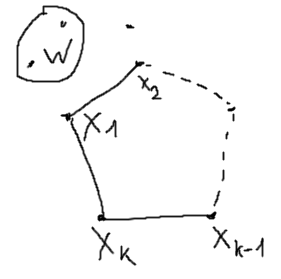
\includegraphics[scale = 0.40]{images/E-H_graph.png}
				\caption{Иллюстрация графа}
\end{wrapfigure} \\
\Proof Предположим противное: в таком графе нет гамильтонового цикла. Тогда рассмотрим любой самый длинный простой цикл $C=\{x_1, ..., x_k\}$. Рассмотрим граф $G'=G \big |_{V \setminus C}$. В $G'$ рассмотрим произвольную компоненту связности $W$. 

\textbf{Множество соседей $W$ в графе $G$} $-$ $N_W(G)= \newline \left \{ y \in V \setminus W : \exists x \in W\left( (x, y) \in E \right) \right \}$.

\underline{Утв. 1}: $N_W(G) \subset C$.

\underline{Утв. 2}: Соседние вершины $C$ не могут принадлежать $N_W(G)$ одновременно (иначе можно удлинить цикл).

\underline{Утв. 3}: $\varkappa(G) \leqslant |N_W(G)|$.

\underline{Утв. 4}: Назовём $M=\{x_{i+1}: x_i \in N_W(G) \}$. По утв. 2 \newline
$M \cap N_W(G) = \varnothing$ и $|M|=|N_W(G)|$. Тогда $M$ $-$ независимое множество вершин. \\
Док-во утв. 4: Предположим противное: в $M$ есть рёбра между вершинами. Тогда выберем в цикле вершины $x_i, x_{i+1}, x_j, x_{j+1}$, при этом между $x_{i+1}$ и $x_{j+1}$ есть ребро.
Тогда можно удлинить цикл: вместо $x_1\!\! \shortrightarrow\!\! x_2\!\! \shortrightarrow\!\! ...\!\! \shortrightarrow\!\! x_i\!\! \shortrightarrow\!\! x_{i+1}\!\! \shortrightarrow\!\! ...\!\! \shortrightarrow\!\! x_j\!\! \shortrightarrow\!\! x_{j+1}\!\! \shortrightarrow\!\! ...\!\! \shortrightarrow\!\! x_k\!\! \shortrightarrow\!\! x_1$ новый цикл $x_1\!\! \shortrightarrow\!\! x_2\!\! \shortrightarrow\!\! ...\!\! \shortrightarrow\!\! x_i\!\! \shortrightarrow\!\! a\!\! \shortrightarrow\!\! ...\!\! \shortrightarrow\!\! b\!\! \shortrightarrow\!\! x_j\!\! \shortrightarrow\!\! ...\!\! \shortrightarrow\!\! x_{i+1}\!\! \shortrightarrow x_{j+1}\!\! \shortrightarrow\!\! ...\!\! \shortrightarrow\!\! x_k\!\! \shortrightarrow\!\! x_1$ ($a, b \in W$). будет как минимум на 1 вершину длиннее, что противоречит предположению, что $C$ - наидлиннейший.

\underline{Утв. 5}: Пусть $x \in W$. Тогда $M \bigcup {x}$ $-$ независимое множество.

Тогда из утв. 5 $\alpha(G) \geqslant |M|+1$, но из утв. 3 $\varkappa(G) \leqslant |M|$. Значит, $\varkappa(G) < \alpha(G)$, что противоречит условию теоремы. \EndProof
\begin{center}
    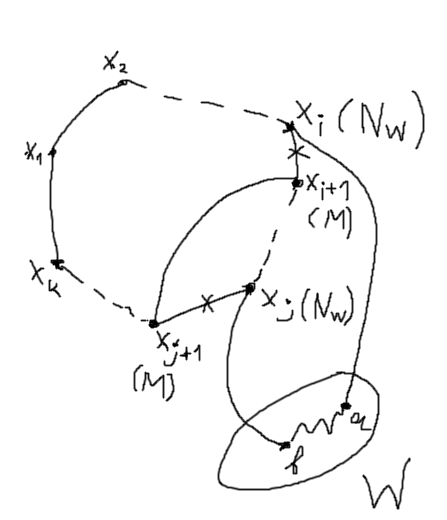
\includegraphics[scale = 0.40]{images/E-H_cycle_lengthening.png}
\end{center}